
\documentclass{article}

\usepackage{fullpage,latexsym,picinpar,amsmath,amsfonts, graphicx, tikz}

           

%%%%%%%%%%%%%%%%%%%%%%%%%%%%%%%%%%%%%%%%%%%%%%%%%%%%%%%%%%%%%%%%%%%%%%%%%%%%%%%%%%%
%%%%%%%%%%%  LETTERS 
%%%%%%%%%%%%%%%%%%%%%%%%%%%%%%%%%%%%%%%%%%%%%%%%%%%%%%%%%%%%%%%%%%%%%%%%%%%%%%%%%%%

\newcommand{\barx}{{\bar x}}
\newcommand{\bary}{{\bar y}}
\newcommand{\barz}{{\bar z}}
\newcommand{\bart}{{\bar t}}

\newcommand{\bfP}{{\bf{P}}}

%%%%%%%%%%%%%%%%%%%%%%%%%%%%%%%%%%%%%%%%%%%%%%%%%%%%%%%%%%%%%%%%%%%%%%%%%%%%%%%%%%%
%%%%%%%%%%%%%%%%%%%%%%%%%%%%%%%%%%%%%%%%%%%%%%%%%%%%%%%%%%%%%%%%%%%%%%%%%%%%%%%%%%%
                                                                                
\newcommand{\parend}[1]{{\left( #1  \right) }}
\newcommand{\spparend}[1]{{\left(\, #1  \,\right) }}
\newcommand{\angled}[1]{{\left\langle #1  \right\rangle }}
\newcommand{\brackd}[1]{{\left[ #1  \right] }}
\newcommand{\spbrackd}[1]{{\left[\, #1  \,\right] }}
\newcommand{\braced}[1]{{\left\{ #1  \right\} }}
\newcommand{\leftbraced}[1]{{\left\{ #1  \right. }}
\newcommand{\floor}[1]{{\left\lfloor #1\right\rfloor}}
\newcommand{\ceiling}[1]{{\left\lceil #1\right\rceil}}
\newcommand{\barred}[1]{{\left|#1\right|}}
\newcommand{\doublebarred}[1]{{\left|\left|#1\right|\right|}}
\newcommand{\spaced}[1]{{\, #1\, }}
\newcommand{\suchthat}{{\spaced{|}}}
\newcommand{\numof}{{\sharp}}
\newcommand{\assign}{{\,\leftarrow\,}}
\newcommand{\myaccept}{{\mbox{\tiny accept}}}
\newcommand{\myreject}{{\mbox{\tiny reject}}}
\newcommand{\blanksymbol}{{\sqcup}}
                                                                                                                         
\newcommand{\veps}{{\varepsilon}}
\newcommand{\Sigmastar}{{\Sigma^\ast}}
                           
\newcommand{\half}{\mbox{$\frac{1}{2}$}} 
\newcommand{\onefourth}{\mbox{$\frac{1}{3}$}}      
\newcommand{\threehalfs}{\mbox{$\frac{3}{2}$}}   
\newcommand{\domino}[2]{\left[\frac{#1}{#2}\right]}  

%%%%%%%%%%%% complexity classes

\newcommand{\PP}{\mathbb{P}}
\newcommand{\NP}{\mathbb{NP}}
\newcommand{\PSPACE}{\mathbb{PSPACE}}
\newcommand{\coNP}{\textrm{co}\mathbb{NP}}
\newcommand{\DLOG}{\mathbb{L}}
\newcommand{\NLOG}{\mathbb{NL}}
\newcommand{\NL}{\mathbb{NL}}

%%%%%%%%%%% decision problems

\newcommand{\PCP}{\sc{PCP}}
\newcommand{\Path}{\sc{Path}}
\newcommand{\GenGeo}{\sc{Generalized Geography}}

\newcommand{\malytm}{{\mbox{\tiny TM}}}
\newcommand{\malycfg}{{\mbox{\tiny CFG}}}
\newcommand{\Atm}{\mbox{\rm A}_\malytm}
\newcommand{\complAtm}{{\overline{\mbox{\rm A}}}_\malytm}
\newcommand{\AllCFG}{{\mbox{\sc All}}_\malycfg}
\newcommand{\complAllCFG}{{\overline{\mbox{\sc All}}}_\malycfg}
\newcommand{\complL}{{\bar L}}
\newcommand{\TQBF}{\mbox{\sc TQBF}}
\newcommand{\SAT}{\mbox{\sc SAT}}

%%%%%%%%%%%%%%%%%%%%%%%%%%%%%%%%%%%%%%%%%%%%%%%%%%%%%%%%%%%%%%%%%%%%%%%%%%%%%%%%%%%
%%%%%%%%%%%%%%% for homeworks
%%%%%%%%%%%%%%%%%%%%%%%%%%%%%%%%%%%%%%%%%%%%%%%%%%%%%%%%%%%%%%%%%%%%%%%%%%%%%%%%%%%

\newcommand{\student}[2]{%
{\noindent\Large{ \emph{#1} SID {#2} } \hfill} \vskip 0.1in}

\newcommand{\assignment}[1]{\medskip\centerline{\large\bf CS 111 ASSIGNMENT {#1}}}

\newcommand{\duedate}[1]{{\centerline{due {#1}\medskip}}}     

\newcounter{problemnumber}                                                                                 

\newenvironment{problem}{{\vskip 0.1in \noindent
              \bf Problem~\addtocounter{problemnumber}{1}\arabic{problemnumber}:}}{}

\newcounter{solutionnumber}

\newenvironment{solution}{{\vskip 0.1in \noindent
             \bf Solution~\addtocounter{solutionnumber}{1}\arabic{solutionnumber}:}}
				{\ \newline\smallskip\lineacross\smallskip}

\newcommand{\lineacross}{\noindent\mbox{}\hrulefill\mbox{}}

\newcommand{\decproblem}[3]{%
\medskip
\noindent
\begin{list}{\hfill}{\setlength{\labelsep}{0in}
                       \setlength{\topsep}{0in}
                       \setlength{\partopsep}{0in}
                       \setlength{\leftmargin}{0in}
                       \setlength{\listparindent}{0in}
                       \setlength{\labelwidth}{0.5in}
                       \setlength{\itemindent}{0in}
                       \setlength{\itemsep}{0in}
                     }
\item{{{\sc{#1}}:}}
                \begin{list}{\hfill}{\setlength{\labelsep}{0.1in}
                       \setlength{\topsep}{0in}
                       \setlength{\partopsep}{0in}
                       \setlength{\leftmargin}{0.5in}
                       \setlength{\labelwidth}{0.5in}
                       \setlength{\listparindent}{0in}
                       \setlength{\itemindent}{0in}
                       \setlength{\itemsep}{0in}
                       }
                \item{{\em Instance:\ }}{#2}
                \item{{\em Query:\ }}{#3}
                \end{list}
\end{list}
\medskip
}

%%%%%%%%%%%%%%%%%%%%%%%%%%%%%%%%%%%%%%%%%%%%%%%%%%%%%%%%%%%%%%%%%%%%%%%%%%%%%%%%%%%
%%%%%%%%%%%%% for quizzes
%%%%%%%%%%%%%%%%%%%%%%%%%%%%%%%%%%%%%%%%%%%%%%%%%%%%%%%%%%%%%%%%%%%%%%%%%%%%%%%%%%%

\newcommand{\quizheader}{ {\large NAME: \hskip 3in SID:\hfill}
                                \newline\lineacross \medskip }


%%%%%%%%%%%%%%%%%%%%%%%%%%%%%%%%%%%%%%%%%%%%%%%%%%%%%%%%%%%%%%%%%%%%%%%%%%%%%%%%%%%
%%%%%%%%%%%%% for final
%%%%%%%%%%%%%%%%%%%%%%%%%%%%%%%%%%%%%%%%%%%%%%%%%%%%%%%%%%%%%%%%%%%%%%%%%%%%%%%%%%%

\newcommand{\namespace}{\noindent{\Large NAME: \hfill SID:\hskip 1.5in\ }\\\medskip\noindent\mbox{}\hrulefill\mbox{}}



\newcommand{\plain}{\node[shape = circle, draw = black]}

\begin{document}

\centerline{\large \bf CS141 Homework 5}

\vspace{0.5in}


%%%%%%%%%%%%%%%%%%%%%%%%%%%%%%%%%%%%%%%%%%%%%%%%%%%%%%%%%%%%%%%%%%%%%%%%%%%%%%%%%%%% Unfinished %%%%%%%%%%%%%%%%%%%%%%%%%%%%%%%%%%%%%%%%%%%%%%%%%%%%%%%%%%%%%%%%%%%%%%%%%%%%%%%%%%%%%%%%%%%%
%%%%%%%%%%%%%%%%%%%%%%%%%%%%%%%%%%%%%%%%%%%%%%%%%%%%%%%%%%%%%%%%%%%%%%%%%%%%%%%%%%%% Problem 1 %%%%%%%%%%%%%%%%%%%%%%%%%%%%%%%%%%%%%%%%%%%%%%%%%%%%%%%%%%%%%%%%%%%%%%%%%%%%%%%%%%%%%%%%%%%%%


\begin{problem} \textit{Pouring water.}

We have three containers whose sizes are $10$ pints, $7$ pints, and $4$ pints, respectively.
The $7$-pint and $4$-pint containers start out full of water, but the $10$-pint container is initially empty. We are allowed one type of operation: pouring the contents of one container into another, stopping only when the source container is empty or the destination container is full. We want to know if there is a sequence of pourings that leaves exactly $2$ pints in the $7$- or $4$-pint container.

\begin{itemize}
	\item[a)] Model this as a graph problem: give a precise deifinition of the graph involved and state the specific question about this graph that needs to be answered.
	\item[b)] What algorithm should be applied to solve the problem?
	\item[c)] Find the answer by applying the algorithm.
\end{itemize}

\end{problem}
\begin{solution}
\begin{itemize}
	\item[a)] We can consider this to be a graph problem where each of the vertices are triples of positive (including zero) whole numbers with (without loss of generality) the first corresponding to the amount of water in the $10$ pint container, the second corresponding to the amount of water in the $7$ pint container, and the third corresponding to the amount of water in the $4$ pint container.  We can then consider that the amount of water in the container ranges between $0$ and the capacity of that specific container such that the first value in the triple ranges from $0$ to $10$, the second value in the triple ranges from $0$ to $7$, and the third value in the triple ranges from $0$ to $4$.  Considering that the water in the set of containers is constant, we can also impose the condition that $t+s+f=11$.  These conditions define a finite set of vertices for our graph.  These statements can be condensed in the following form:
	$$V=\{(t,s,f)| t,s,f \in \mathbb{Z}^+_0, 0 \leq t \leq 10, 0 \leq s \leq 7, 0 \leq f \leq 4, t+s+f=11\}$$
	Now that the set of vertices in our graph has been well defined, lets consider what edges are possible in the graph.  In a sense, there are two "types" of edges in this graph, one corresponding to each stopping condition in the one allowed move.  In all of the edges, the sum of all values in the triple remains constant at 11 and 
	\item[b)] BFS or DFS can both be used to solve this problem.
	\item[c)] 
\end{itemize}
\end{solution}


%%%%%%%%%%%%%%%%%%%%%%%%%%%%%%%%%%%%%%%%%%%%%%%%%%%%%%%%%%%%%%%%%%%%%%%%%%%%%%%%%%%% Finished %%%%%%%%%%%%%%%%%%%%%%%%%%%%%%%%%%%%%%%%%%%%%%%%%%%%%%%%%%%%%%%%%%%%%%%%%%%%%%%%%%%%%%%%%%%%%%
%%%%%%%%%%%%%%%%%%%%%%%%%%%%%%%%%%%%%%%%%%%%%%%%%%%%%%%%%%%%%%%%%%%%%%%%%%%%%%%%%%%% Problem 2 %%%%%%%%%%%%%%%%%%%%%%%%%%%%%%%%%%%%%%%%%%%%%%%%%%%%%%%%%%%%%%%%%%%%%%%%%%%%%%%%%%%%%%%%%%%%%


\begin{problem}

If there is ever a decision between multiple neighbor nodes in the BFS or DFS algorithms, assume we always choose the letter in alphabetical order.


\begin{itemize}
	\item[a)]{} Consider the following adjacency matrix:
		\begin{figure}[h!]
			\centering
			%\includegraphics[width=4.5in]{graph4a.pdf}
		\end{figure}
		
		\begin{itemize}
			\item[a.1)]{} Draw the graph that is represented by the matrix.
			\item[a.2)]{} In what order will the nodes be visited using Breadth First Search?
			\item[a.3)]{} In what order will the nodes be visited using Depth First Search?
		\end{itemize}
	\item[b)]{} If you have the $0/1$ adjacency matrix of a graph and you take the matrix to the $N^{th}$ power, thent he $(i,j)^{th}$ entry of the result tells how many paths of length $N$ there are from vertex $i$ to vertex $j$ (here, the length is measured in number of edges traversed).  For example, in a), according to the adjacency matrix, there is a path of length $1$ edge between vertices $A$ and $B$.
		\vskip 0.15in
		Let $G = (V,E)$ be an undirected graph.  A triangle in $G$ is a cycle consisting of exactly three vertices (or, equivalently, three edges).  Suppose that $G$ is represented as an adjacency matrix.  Give an algorithm to determine whether $G$ contains any triangle in $O(n^{\log_2{7}})$ worst-case time.
	\item[c)]{} Using matrix multiplications, find all the triangles in the graph, represented by the following adjacency matrix:
		\begin{figure}[h!]
			\centering
			%\includegraphics[width=3.6in]{graph4c.pdf}
		\end{figure}
\end{itemize}
\end{problem}
\begin{solution}

\begin{itemize}
	\item[a)]{} It is useful to note that the adjacency matrix, which I will call $mat(G)$, the matrix is symmetric about its proper diagonal ($mat(G)^T=mat(G)$), and therefore, it represents an undirected graph.
		\begin{itemize}
			\item[a.1)]{} The (undirected) graph represented by this adjacency matrix can be drawn as follows:
				\vskip 0.15in
				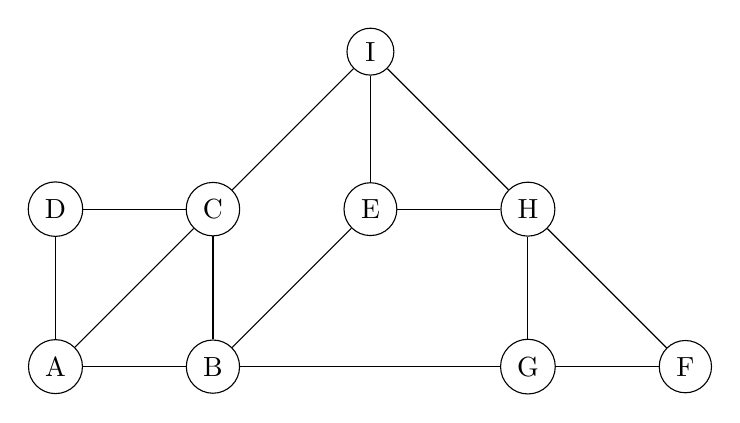
\begin{tikzpicture}
					\plain (a) at (0,0) {A};
					\plain (b) at (2,0) {B};
					\plain (c) at (2,2) {C};
					\plain (d) at (0,2) {D};
					\plain (e) at (4,2) {E};
					\plain (f) at (8,0) {F};
					\plain (g) at (6,0) {G};
					\plain (h) at (6,2) {H};
					\plain (i) at (4,4) {I};
					\path (a) edge (b) edge (c) edge (d);
					\path (b) edge (c) edge (e) edge (g);
					\path (c) edge (d) edge (i);
					\path (e) edge (i) edge (h);
					\path (f) edge (h) edge (g);
					\path (g) edge (h);
					\path (h) edge (i);
				\end{tikzpicture}
			\item[a.2)]{} The edges would be visited in the order A, B, C, D, E, G, I, H, F if we were to search the graph with BFS.
			\item[a.3)]{} The edgew would be visited in the order A, B, E, H, F, G, I, C, D if we were to search the graph with DFS.
		\end{itemize}
	\item[b)]{} There are a few things to note about a cycle (in this case, a triangle).  Consider that a cycle is can always be thought of as a path from a node to itself.  This means that for any length N, all cycles of length N are counted at least once in the diagonal elements of the matrix.  We can also note that those cycles of length N are double counted, considering that there are two orderings for the vertices that we traverse (clockwise and counterclockwise, if you like).  Additionally, all cycles of length N are counted twice for each vertex in the graph - that is N times each.  Therefore, the trace of the $0/1$ adjacency matrix for a given graph raised to the $N^{th}$ power is exactly equal to $2N$ times the nubmer of cycles of that length.  Mathematically, this corresponds to the equation $tr(mat(G)^N)=2NC$ where $C$ is the number of cycles of length $N$.  We can rearrange this equation to give $C=\frac{tr(mat(G)^N)}{2N}$.  Now, recall the Strassen algorithm for matrix multiplication.  If we apply this agorithm three times to $mat(G)$ (each time, multiplying the previous product by $mat(G)$), we can efficiently calculate $mat(G)^3$ (by efficiently, I mean that the runtime would be $O(n^{\log_2(7)})$). Now, using the previously stated formula, we can then calculate the number of triangles in linear time, as calculating the trace of an $n \times n$ matrix in $O(n)$ time by simply adding the diagonals.  Since calculating the trace is faster than matrix multiplication, we can ignore its impact on the runtime and write the overall runtime as $O(n^{\log_2(7)})$.
	\item[c)]{}  In order to calculate the number of triangles in the given graph using matrix multiplications, we first need a few things.  $N$, in this case would be 3, and so $2N = 6$.  We next need to calculate $mat(G)^N = mat(G)^3$ which turns out to be:
		\vskip 0.15in
		\begin{tabular}{|c|c|c|c|c|c|c|c|c|c|c|c|c|c|c|c|c|c|c|c|c|c|c|c|c|c|c|c|c|c|c|c|c}
			\hline
			   & A & B & C & D & E & F & G\\
			\hline
			 A & 4 & 6 & 6 & 6 & 2 & 3 & 1\\
			\hline
			 B & 6 & 2 & 7 & 2 & 3 & 4 & 3\\
			\hline
			 C & 6 & 7 & 4 & 8 & 1 & 6 & 1\\
			\hline
			 D & 6 & 2 & 8 & 2 & 5 & 1 & 2\\
			\hline
			 E & 2 & 3 & 1 & 5 & 0 & 4 & 0\\
			\hline
			 F & 3 & 1 & 6 & 1 & 4 & 0 & 1\\
			\hline
			 G & 1 & 3 & 1 & 2 & 0 & 1 & 0\\
			 \hline
		\end{tabular}
		\vskip 0.15in
		We can then calculate the trace as $4+2+4+2+0+0+0 = 12$, then divide the trace by 6 to give that there are 2 triangles in the graph.
\end{itemize}

\end{solution}


%%%%%%%%%%%%%%%%%%%%%%%%%%%%%%%%%%%%%%%%%%%%%%%%%%%%%%%%%%%%%%%%%%%%%%%%%%%%%%%%%%%% Unfinished %%%%%%%%%%%%%%%%%%%%%%%%%%%%%%%%%%%%%%%%%%%%%%%%%%%%%%%%%%%%%%%%%%%%%%%%%%%%%%%%%%%%%%%%%%%%
%%%%%%%%%%%%%%%%%%%%%%%%%%%%%%%%%%%%%%%%%%%%%%%%%%%%%%%%%%%%%%%%%%%%%%%%%%%%%%%%%%%% Problem 3 %%%%%%%%%%%%%%%%%%%%%%%%%%%%%%%%%%%%%%%%%%%%%%%%%%%%%%%%%%%%%%%%%%%%%%%%%%%%%%%%%%%%%%%%%%%%%


\begin{problem} 

You are given a directed graph $G = (V, E)$, where $V = \{1, \ldots , n\}$, i.e., the vertices are integers in the range $1$ to $n$. For every vertex $i$ we would like to compute the value $m(i)$ defined as follows: $m(i)$ is the smallest $j$ such that vertex $j$ is reachable from vertex $i$. (As a convention, we assume that $i$ is reachable from $i$.) Show that the values $m(1), \ldots , m(n)$ can be computed in $O(|V | + |E|)$ time.
\end{problem}
\begin{solution}
\end{solution}


%%%%%%%%%%%%%%%%%%%%%%%%%%%%%%%%%%%%%%%%%%%%%%%%%%%%%%%%%%%%%%%%%%%%%%%%%%%%%%%%%%%% Finished %%%%%%%%%%%%%%%%%%%%%%%%%%%%%%%%%%%%%%%%%%%%%%%%%%%%%%%%%%%%%%%%%%%%%%%%%%%%%%%%%%%%%%%%%%%%%%
%%%%%%%%%%%%%%%%%%%%%%%%%%%%%%%%%%%%%%%%%%%%%%%%%%%%%%%%%%%%%%%%%%%%%%%%%%%%%%%%%%%% Problem 4 %%%%%%%%%%%%%%%%%%%%%%%%%%%%%%%%%%%%%%%%%%%%%%%%%%%%%%%%%%%%%%%%%%%%%%%%%%%%%%%%%%%%%%%%%%%%%


\begin{problem}

You are given a set of cities, along with the pattern of highways between them, in the form of an undirected graph $G=(V,E)$. Each stretch of highway $e\in E$ connects two of the cities, and you know its length in miles $l_e$. You want to get from city $s$ to city $t$. There's one problem: your car can only hold enough gas to cover $L$ miles. There are gas stations in each city, but not between cities. Therefore, you can only take a route if every one of its edges has length $l_e \leq L$.
\begin{itemize}
	\item[a)]{} Given the limitation on your car's fuel tank capacity, show how to determine, in linear time, whether there is a feasible route form $s$ to $t$.
	\item[b)]{} You are now planning to buy a new car, and you want to know the minimum fuel tank capacity that is needed to travel from $s$ to $t$.  Give an $O((\mid V \mid + \mid E \mid) \log {\mid V \mid})$ algorithm to determine this.
\end{itemize}
\end{problem}

\begin{solution}
\begin{itemize}
	\item[a)]{} I will assume, for the rest of this problem, that the edges in this graph (the highways between cities) are given in the form of an adjacency matrix.  This is for the fact that there are no parallel edges (edges between the same two vertices) in an adjacency matrix and this simplifies the problem.  However, in the case that the edges are not given in the form of an adjacency matrix, it is fairly simple to map the edges to an adjacency matrix by eliminating parallel edges through only considering the shortest edge (highway) between any two given cities.  Now, considering that we have the edges listed in an adjacency matrix, we can apply a clamping function to transform it into a $0/1$ adjacency matrix.  This effectively entails iterating over each edge and setting it to 1 if it is less than the length that we can drive and 0 if it is longer than we can drive.  Now, we effectively have a $0/1$ adjacency matrix that represents which roads we can and cannot travel on, and we can actually begin our algorithm. Note, however that each of these operations is linear with respect to the number of edges that are in the graph ($|E|$) and so we have not yet exceeded the runtime allocation of this problem.  Now, we can consider applying BFS or DFS to this matrix (which both run in $O(|V|+|E|)$) to the $0/1$ matrix that we have constructed and by doing so, find a feasible route from any vertex to another in linear time.
	\item[b)]{} Calculating the minimum fuel tank capacity required to travel from $s$ to $t$ is equivalent to calculating the maximum edge length needed to take in the path from $s$ to $t$.  The runtime allocation in the problem is somewhat illustrative of what algorithm we need to use (or modify) in order to solve the problem.  Dijkstra's algorithm has a running time of $O((\mid V \mid + \mid E \mid) \log {\mid V \mid})$, so if we could modify it in some way to accurately calculate the longest individual edge length in the path from $s$ to $t$, we can solve this problem.  The first method for which we could try to calculate the minimum tank capacity required is by adding back tracking to our Dijkstra's implementation and using it to find the maximal edge length in our path from $s$ to $t$.  This seems promising, but it is flawed.  Dijkstra's algorithm as it is normally implemented optimized the overall path length, not the individual edge lengths used in the path.  Through this approach, we are not guaranteed that the path that we have found actually minimizes the fuel tank required, so we must consider another method.  Now, we can consider extending a path from $v'$ to $v$, the maximum edge length in the path from $s$ to $v$, $m(v)$ is equal to $max(l(v',v),m(v'))$.  Now, we can use this recursion in this specific implementation of Dijkstra's algorithm to obtain, in $O((\mid V \mid + \mid E \mid) \log {\mid V \mid})$ time, the minimal tank capacity required to get from $s$ to $t$.
\end{itemize}
\end{solution}

\newpage


%%%%%%%%%%%%%%%%%%%%%%%%%%%%%%%%%%%%%%%%%%%%%%%%%%%%%%%%%%%%%%%%%%%%%%%%%%%%%%%%%%%% Unfinished %%%%%%%%%%%%%%%%%%%%%%%%%%%%%%%%%%%%%%%%%%%%%%%%%%%%%%%%%%%%%%%%%%%%%%%%%%%%%%%%%%%%%%%%%%%%
%%%%%%%%%%%%%%%%%%%%%%%%%%%%%%%%%%%%%%%%%%%%%%%%%%%%%%%%%%%%%%%%%%%%%%%%%%%%%%%%%%%% Problem 5 %%%%%%%%%%%%%%%%%%%%%%%%%%%%%%%%%%%%%%%%%%%%%%%%%%%%%%%%%%%%%%%%%%%%%%%%%%%%%%%%%%%%%%%%%%%%%


\begin{problem} (Extra credit)

Consider the following adjacency matrix:
\begin{figure}[h!]
    \centering
    %\includegraphics[width = 2.5in]{BellFord}
\end{figure}
\begin{itemize}
	\item[a)]{} Draw the graph that is represented by this matrix.
	\item[b)]{} Apply the Bellman-Ford algorithm to the graph to find the shortest paths from vertex $A$ to all other vertices.  Show every iteration.
	\item[c)]{} Does this graph have negative cycles?
\end{itemize}
\end{problem}

\begin{solution}
\end{solution}

%%%%%%%%%%%%%%%%%




\end{document}
